\documentclass[11pt]{article}
\title{Zusammenfassung Numerik 2022 WS}
\author{Simon Garger}
\usepackage{amsmath}
\usepackage{amssymb}
\usepackage{amsfonts}
\usepackage{setspace}
\usepackage{fullpage}
\usepackage{blkarray}
\usepackage[a4paper,left=2.5cm,right=2.5cm,top=2cm,bottom=4cm,bindingoffset=5mm]{geometry}
\usepackage{graphicx}
\usepackage{wasysym}
\usepackage{mathtools}
\usepackage{titlesec}
\usepackage{xcolor}
\usepackage{bm}
\usepackage{enumitem}
\usepackage{amsbooka}
\usepackage{translit}
\usepackage{arabicore}
\usepackage{amsmath-2018-12-01}
\usepackage{amsmath-2018-12-01}
\usepackage{farsifnt}


\newcommand{\N}{\mathbb{N}}
\newcommand{\Z}{\mathbb{Z}}
\newcommand{\R}{\mathbb{R}}
\newcommand{\C}{\mathbb{C}}
\newcommand{\res}{\text{res}}
\renewcommand{\Re}{\mathfrak{Re}}
\renewcommand{\Im}{\mathfrak{Im}}


\newenvironment{problem}[2][Beispiel]{
    \begin{trivlist}
        \item[\hskip \labelsep {\bfseries #1}\hskip \labelsep {\bfseries #2.}] \itshape}{
    \end{trivlist}\normalshape
}

\begin{document}
    \begin{problem}{1}
        $\quad$
        \begin{enumerate}[label = (\roman{enumi})]
            \item Seien $f:S^1\to\C$ und $g:\R\to\C$ die $2\pi$-periodische Funktion $g(x):=f(e^{ix})$. Zeigen Sie,
            dass $f$ stetig ist, genau dann wenn $g$ stetig ist.
            \item Zeigen Sie, dass für jede $2\pi$-periodische und stetige Funktion $g:\R\to\C$ eine stetige
            Funktion $f:S^1\to\C$ existiert, mit $g(x)=f(e^{ix})$ für jedes $x\in \R$.
        \end{enumerate}
        (Hier, $S^1:= \{z\in\C:|z|=1\}$.)
    \end{problem}

    \begin{proof}
        Ist $f$ stetig, so ist $g$ als Zusammensetzung stetiger Funktionen stetig. Ist hingegen
        $g$ stetig und $z_n\to z$ eine Konvergente Folge auf $S^1$. Dann finden wir eine Folge
        $\theta_n\to\theta$ mit $e^{i\theta_n}=z_n$ und $e^{i\theta}=z$. Denn nehmen wir an, das
        wäre nicht der Fall, dann würden wir eine Teilfolge $\theta_{n_k}$ finden, die nicht gegen $\theta$ sondern
        gegen $\tilde{\theta}$ (mit $\theta\neq \tilde{\theta}\mod 2\pi$) konvergiert (weil $S^1$
        kompakt ist). Dann gilt aber $|z_{n_k}-z|=\left|e^{i\theta_{n_k}}-e^{i\theta}\right|\nrightarrow 0$.
        Damit finden wir nun für die Folge $z_n$:
        $$\lim_{n\to\infty}f(z_n)=\lim_{n\to\infty} f(e^{i\theta_n}) = \lim_{n\to\infty} g(\theta_n)=
        g(\theta)= f(e^{i\theta})=f(z)$$
        Also haben wir auch die Umkehrung gezeigt. \\\\
        Wir betrachten $g$ für den zweiten Unterpunkt zuerst nur auf $[-\pi,\pi]$. Dann definieren wir
        $f$ durch $f(z)=f(e^{i\theta}):= g(\theta)$. Dabei schreiben wir $z$ immer mit $\theta\in [-\pi,\pi]$.
        Sei nun $\alpha:= \theta + 2k\pi$ beliebig:
        $$g(\alpha) = g(\theta + 2k\pi)=g(\theta)=f(e^{i\theta})=f(e^{i\theta}\cdot e^{2k\pi})=
        f(e^{i\alpha})$$
        Also erfüllt unser $f$ die Bedingung $g(x)=f(e^{ix})$. Weiter wissen wir, aus Punkt $1$, dass
        $f$ stetig ist.
    \end{proof}

    \begin{problem}{2}
        Betrachten Sie die $2\pi$-periodische ungerade Funktion, die auf $[0,\pi]$ durch $f(x)=x(\pi-x)$
        definiert ist.
        \begin{enumerate}[label = (\roman{enumi})]
            \item Zeichnen Sie den Graphen von $f$.
            \item Berechnen Sie die Fourier-Koeffizienten von $f$ und zeigen Sie, dass:
            $$f(x)=\frac{8}{\pi}\sum_{k\geq 1\text{  ungerade}}\frac{\sin(kx)}{k^3},\qquad x\in\R.$$
        \end{enumerate}
    \end{problem}

    \begin{proof}
        Wir zeichnen die Funktion im Intervall $[0,\pi]$ und setzen sie zuerst ungerade und dann
        periodisch fort. Damit erhalten wir
        \begin{figure}
            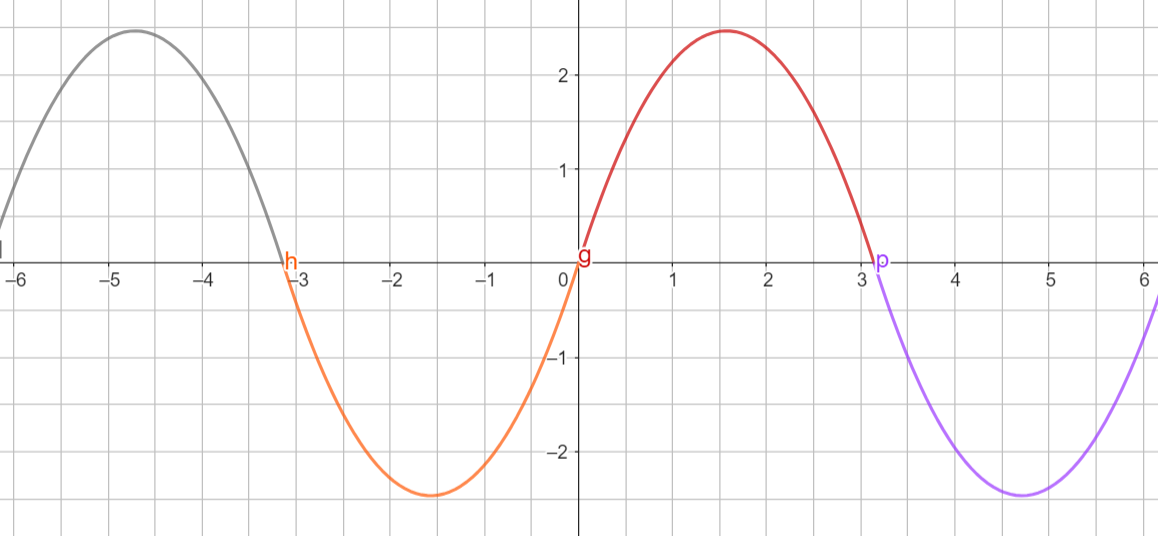
\includegraphics[width=\linewidth]{Unbenannt.PNG}
            \caption{f(x)}
        \end{figure}
        Nun bestimmen wir die Fourierkoeffizienten für $n\neq 0$:
        $$\begin{aligned}
              2\pi\hat{f}(n) &= \int_{-\pi}^0 x(\pi+x)e^{-inx}dx + \int^{\pi}_0 x(\pi-x)e^{-inx}dx\\
              &= \int_{-\pi}^0 \pi xe^{-inx}dx +\int_{-\pi}^0 x^2e^{-inx}dx +
              \int^{\pi}_0 \pi x e^{-inx}dx-\int^{\pi}_0 x^2e^{-inx}dx\\
              &= \int^{\pi}_{-\pi} \pi x e^{-inx}dx+\int_{-\pi}^0 x^2e^{-inx}dx-\int^{\pi}_0 x^2e^{-inx}dx
        \end{aligned}$$
        Wir berechnen die zugehörigen Stammfunktionen durch partielles Integrieren:
        $$\int\pi xe^{-inx}dx = \frac{\pi xe^{-inx}}{-in}-\frac{\pi}{-in}\int e^{-inx}dx =
        \frac{\pi xe^{-inx}}{-in}+\frac{\pi}{n^2}e^{-inx}$$
        und
        $$\int x^2e^{-inx}dx=\frac{x^2 e^{-inx}}{-in}-\frac{2}{-in}\int xe^{-inx}dx =
        \frac{x^2 e^{-inx}}{-in}+\frac{2}{in}\cdot\frac{ xe^{-inx}}{-in}+\frac{2}{in}\cdot
        \frac{1}{n^2}e^{-inx}$$
        Wir setzen die Grenzen ein:
        $$\begin{aligned}
              &\phantom{=}\int^{\pi}_{-\pi} \pi x e^{-inx}dx+\int_{-\pi}^0 x^2e^{-inx}dx-
              \int^{\pi}_0 x^2e^{-inx}dx\\
              &= \frac{\pi^2 e^{-in\pi}}{-in}+\frac{\pi e^{-in\pi}}{n^2}+\frac{\pi^2 e^{-in\pi}}{-in}-
              \frac{\pi e^{-in\pi}}{n^2}+\\&\frac{2}{in^3}+\frac{\pi^2 e^{in\pi}}{in}+
              \frac{2\pi e^{in\pi}}{n^2}-\frac{2e^{in\pi}}{in^3} +\\&
              \frac{\pi^2 e^{in\pi}}{in}-\frac{2\pi e^{in\pi}}{n^2}-
              \frac{2e^{-in\pi}}{in^3}+\frac{2}{in^3}\\
              &=-\frac{4i}{n^3}+\frac{4 ie^{-in\pi}}{n^3} = \frac{4i((-1)^n-1)}{n^3}
        \end{aligned}$$
        Also gilt $\hat{f}(n)=\frac{2i((-1)^n-1)}{\pi n^3}$.\\\\
        Für $n=0$ finden wir hingegen:
        $$\begin{aligned}
              \hat{f}(0)&=\int^{\pi}_{-\pi} \pi x dx+\int_{-\pi}^0 x^2dx-
              \int^{\pi}_0 x^2dx\\
              &= \frac{\pi}{2}(\pi^2-\pi^2)-\frac{1}{3}\pi^3+\frac{1}{3}\pi^3 =0
        \end{aligned}$$
        Da die Funktion stetig und periodisch ist, konvergiert die Fourierreihe gegen $f$.
        Damit haben wir insgesamt (mit $\Z^-$ für negative ganze Zahlen und $\Z^+$ für positive):
        $$\begin{aligned}
              f(x)&=\sum_{\Z\setminus\{0\}}\frac{2i((-1)^n-1)}{\pi n^3}e^{inx}\\
              &= \sum_{\Z^-}\frac{2i((-1)^n-1)}{\pi n^3}e^{inx}+ \sum_{\Z^+}\frac{2i((-1)^n-1)}{\pi n^3}e^{inx}\\
              &= \sum_{\Z^+}\frac{2i((-1)^n-1)}{-\pi n^3}e^{-inx}+\sum_{\Z^+}\frac{2i((-1)^n-1)}{\pi n^3}e^{inx}\\
              &= \sum_{\Z^+}\frac{2i((-1)^n-1)}{\pi n^3}(e^{inx}-e^{-inx})\\
              &= \sum_{\Z^+}\frac{2i((-1)^n-1)}{\pi n^3}(e^{inx}-e^{-inx})\\
              &= \sum_{\Z^+, \text{ ungerade}}\frac{-4i}{\pi n^3}(e^{inx}-e^{-inx})\\
              &= \sum_{\Z^+, \text{ ungerade}}\frac{8}{\pi n^3}\left(\frac{e^{inx}-e^{-inx}}{2i}\right)\\
              &= \frac{8}{\pi}\sum_{\Z^+, \text{ ungerade}}\frac{\sin(nx)}{n^3}
        \end{aligned}$$
    \end{proof}
\end{document}